\documentclass[10pt, twoside, openany]{book}

\usepackage[a4paper, top=2.5cm, bottom=2.5cm, left=3cm, right=3cm]{geometry}
\usepackage[utf8]{inputenc}
\usepackage[italian]{babel}
\usepackage{cite}
\usepackage[numbers, sort&compress]{natbib}
\usepackage{hyperref}
\usepackage{graphicx}
\usepackage{fancyhdr}
\usepackage[Lenny]{fncychap}
\usepackage{frontespizio}
\usepackage{tabularx}
\usepackage{caption}

\pagestyle{fancy}
\fancyhead{}
\fancyhead[LE]{\nouppercase{\leftmark}}
\fancyhead[RO]{\nouppercase{\rightmark}}
\bibliographystyle{unsrtnat} %Ordine dei riferimenti bibliografici = ordine con cui le citazioni compaiono nel testo.

\begin{document}
\begin{frontespizio}
\Universita{Roma Tor Vergata}
\Dipartimento{Ingegneria Civile e Ingegneria dell'Informazione}
\Corso{Ingegneria Informatica}
\Annoaccademico{2023/2024}
\Titolo{Titolo della tesi}
\Candidato[0316179]{Matteo Fanfarillo}
\Relatore{Giuseppe Bianchi}
\Correlatore{Francesco Gringoli}
\Logo{logo.png}
\end{frontespizio}

\begin{flushright}
\null\vspace{\stretch{1}}
\textit{[Citazione]}
\vspace{\stretch{2}}\null
\end{flushright}

\tableofcontents
\listoffigures
\listoftables

\chapter{Introduzione}
\section{Panoramica sulla eSIM}
La eSIM (embedded-SIM) non è altro che una SIM virtuale: grazie a lei, quando l'utente vuole cambiare operatore, non deve più acquistare fisicamente una nuova SIM card presso un negozio del nuovo operatore, bensì gli è sufficiente ricevere via e-mail un profilo, ossia una "SIM digitale" che può essere caricata subito sul telefono mediante la scansione di un QR code. Si tratta di una soluzione molto più pratica rispetto a recarsi fisicamente presso il negozio dell'operatore, tant'è vero che negli ultimi anni si sta diffondendo sempre di più: uno studio di Juniper Research stima che il numero di telefoni che utilizzano la connettività eSIM aumenterà dai 986 milioni attuali ai 3.5 miliardi entro il 2027 \cite{Corcom}. Per questi motivi, e poiché le informazioni associate alla comunicazione tra eSIM sono sensibili, è fondamentale garantire un livello di sicurezza sufficientemente elevato per il funzionamento dell'eSIM sia a run-time che a boot-time.

\section{Obiettivo del lavoro}
La presente trattazione si propone di effettuare un'analisi di sicurezza e delle vulnerabilità della eSIM e del suo funzionamento e, successivamente, di tentare di sfruttare, anche con delle attività di laboratorio, le eventuali vulnerabilità trovate.

\section{Definizioni preliminari}
\begin{itemize}
\item \textbf{eUICC (embedded Universal Integrated Circuit Card)}: è un chip utilizzato all'interno dei telefoni all'interno del quale è embeddato il software dell'eSIM. È integrato direttamente nei dispositivi (i.e. non è rimovibile) ed è progettato per essere programmato a distanza. Può contenere uno o più profili eSIM.
\item \textbf{SM-DP+ (Subscription Manager Data Preparation plus)}: è un protocollo che rappresenta una tecnica di provisioning usata per configurare le eSIM in modo automatico e remoto. Rispetto alla versione base SM-DP, offre delle funzionalità aggiuntive come un sistema di crittografia più avanzato e un'architettura di rete più flessibile.
\item \textbf{LPA (Local Profile Assistant)}: è un'applicazione che vive nel telefono dell'utente ed è responsabile della gestione dei profili all'interno della rete mobile, incluse la creazione, l'aggiornamento e la cancellazione.
\end{itemize}

\section{Panoramica sui capitoli successivi}
Nel capitolo 2 verrà svolta una trattazione dettagliata sull'architettura e sulle interfacce dell'eSIM, con lo scopo di fornire al lettore gli strumenti per comprendere appieno le tematiche centrali del lavoro. Nel capitolo 3 verrà effettuata un'analisi della sicurezza dell'eSIM a run-time, mentre nel capitolo 4 si procederà con l'analisi della sicurezza dell'eSIM a boot-time (i.e. durante la fase di configurazione). Infine, nel capitolo 5 verranno mostrati i risultati finali, verranno tratte delle conclusioni sul lavoro svolto e verrà fornita una panoramica sui possibili progetti futuri che potranno essere intrapresi a partire dai risultati ottenuti attraverso questo lavoro.

\chapter{Interfacce e funzionamento dell'eSIM}
\section{Architettura di RSP}
Per comprendere appieno come funziona e come si interfaccia l'eSIM all'interno dei dispositivi mobili, è necessario introdurre il protocollo RSP, anche perché la eSIM si colloca proprio all'interno dell'architettura di RSP.\\
RSP (Remote SIM Provisioning) è un protocollo utilizzato dal protocollo SM-DP+ per gestire la comunicazione tra il server SM-DP+ e la scheda eSIM del dispositivo mobile (i.e. l'eUICC). In particolare, definisce le operazioni di provisioning specifiche per la comunicazione dell'eUICC. Quest'ultimo comprende i dati sia dell'operatore che dell'utente che, nel caso delle SIM tradizionali, verrebbero appunto memorizzati su una SIM card fisica. Entrando più nel dettaglio sul funzionamento di RSP, l'end user che vuole ottenere un profilo eSIM offerto da un particolare operatore (nel quale viene definito un piano tariffario), deve pagare l'operatore affinché esso gli fornisca un codice QR. Dopodiché, deve effettuare la scansione di tale codice QR per avviare lo scaricamento (operazione di Download) e l'installazione (operazione di Install) del profilo eSIM: a questo punto, la connessione tra end user (col relativo profilo eSIM) e operatore è completata. Se in un secondo momento l'end user ha la necessità di ottenere e utilizzare un secondo profilo eSIM, gli è sufficiente ripetere i medesimi passaggi appena descritto, e questo secondo profilo può essere installato all'interno del medesimo eUICC che ospita già il primo profilo. Tale meccanismo è illustrato nella figura \ref{fig:RSP-functioning} tratta da \cite{GSMA-whitepaper}.
\begin{figure}
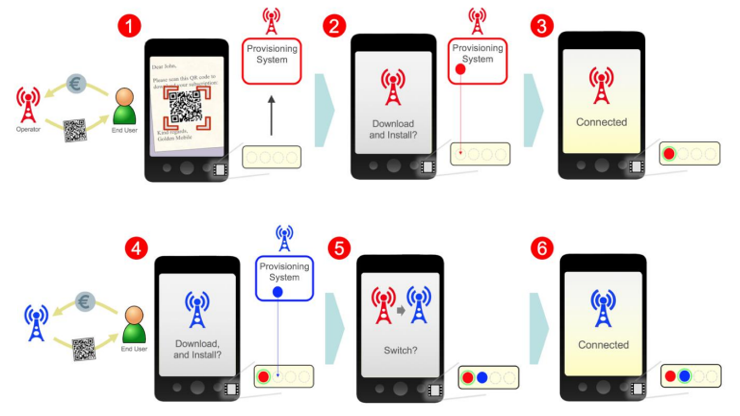
\includegraphics[width=\linewidth]{RSP-functioning.png}
\caption{Comunicazione tra end user e operatore nel contesto del Remote SIM Provisioning.}
\label{fig:RSP-functioning}
\end{figure}
\\Per quanto riguarda l'architettura interna di RSP nello specifico, esistono due soluzioni differenti \cite{GSMA-docs}.
\begin{enumerate}
\item \textbf{LPA embeddato nel dispositivo mobile ma non all'interno dell'eUICC (LPAd)}: oltre alla comunicazione tra l'applicazione LPA e SM-DP+, si utilizzano delle apposite interfacce anche per la comunicazione tra l'eUICC e l'applicazione LPA, come mostrato nella figura \ref{fig:RSP-LPAd} tratta da \cite{GSMA-docs}.
\begin{figure}
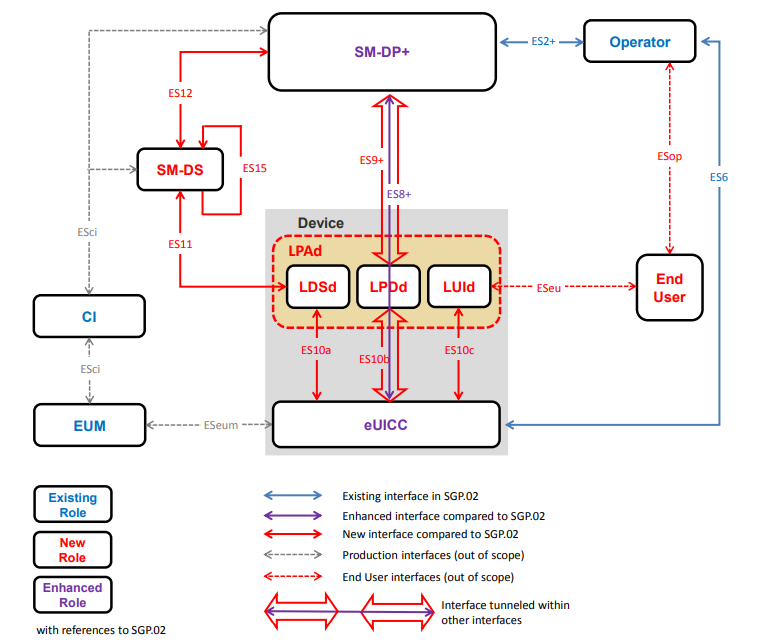
\includegraphics[width=\linewidth]{RSP-LPAd.png}
\caption{Architettura di RSP nel caso di LPA non embeddato nell'eUICC.}
\label{fig:RSP-LPAd}
\end{figure}
Di seguito è riportato un breve glossario che chiarisce il significato di alcuni componenti appartenenti all'architettura di RSP raffigurata in \ref{fig:RSP-LPAd}.
\begin{itemize}
\item \textbf{CI} = Certificate Issuer: è un'entità autorizzata a rilasciare certificati digitali.
\item \textbf{EUM} = eUICC Manufacturer: è il fornitore delle eUICC e del software residente (e.g. firmware, sistema operativo).
\item \textbf{LDSd} = Local Discovery Service (quando LPA non è nell'eUICC).
\item \textbf{LPDd} = Local Profile Download (quando LPA non è nell'eUICC).
\item \textbf{LUId} = Local User Interface (quando LPA non è nell'eUICC).
\item \textbf{SM-DS} = Subscription Manager Discovery Server: è il componente che fornisce un mezzo a SM-DP+ per raggiungere l'eUICC senza dover sapere a quale rete il dispositivo è connesso.
\end{itemize}
\item \textbf{LPA embeddato all'interno dell'eUICC (LPAe)}: sono necessarie solo delle interfacce tra l'eUICC e SM-DP+, come mostrato nella figura \ref{fig:RSP-LPAe} tratta da \cite{GSMA-docs}.
\begin{figure}
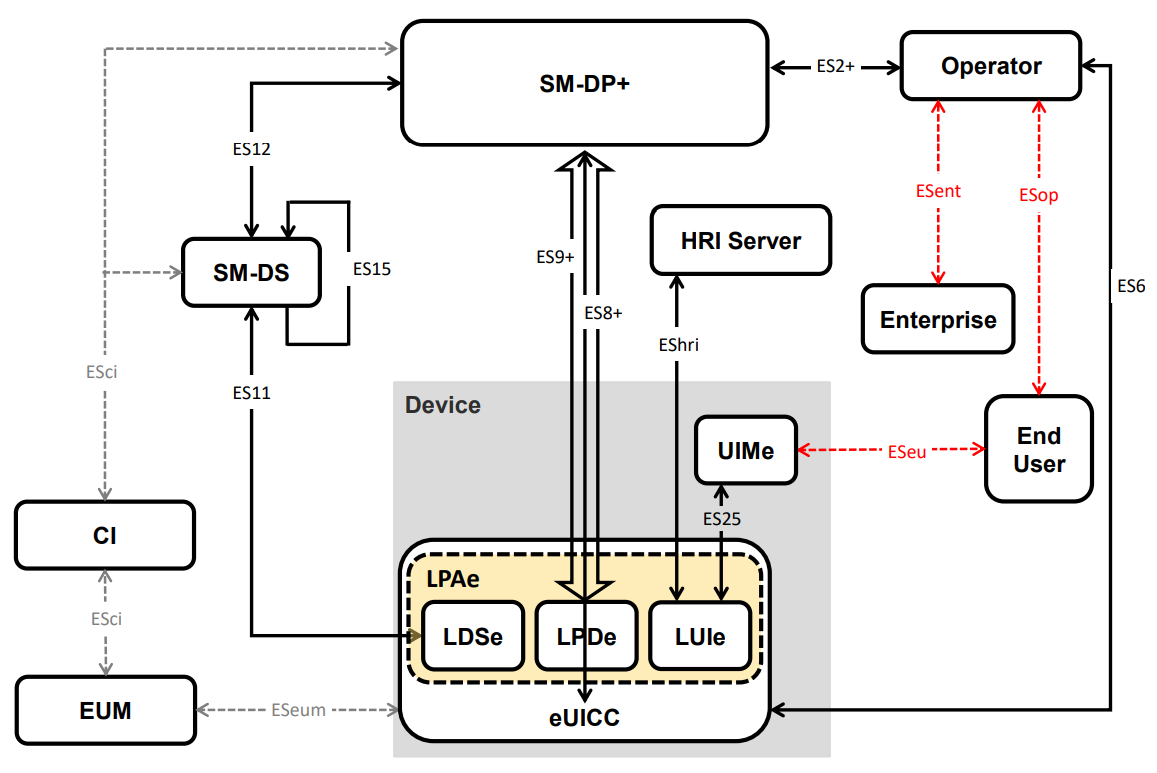
\includegraphics[width=\linewidth]{RSP-LPAe.png}
\caption{Architettura di RSP nel caso di LPA embeddato nell'eUICC.}
\label{fig:RSP-LPAe}
\end{figure}
Successivamente è riportato un breve glossario che chiarisce il significato di alcuni componenti appartenenti all'architettura di RSP raffigurata in \ref{fig:RSP-LPAe}.
\begin{itemize}
\item \textbf{LDSe} = Local Discovery Service (quando LPA è nell'eUICC).
\item \textbf{LPDe} = Local Profile Download (quando LPA è nell'eUICC).
\item \textbf{LUIe} = Local User Interface (quando LPA è nell'eUICC).
\end{itemize}
\end{enumerate}

\subsection{Interfacce presenti nell'architettura di RSP}
Sono illustrate nella tabella \ref{tab:interfaces}, costruita a partire da informazioni tratte da \cite{GSMA-docs}.
\begin{table}[h!]
\begin{center}
\captionsetup{skip=4pt}
\caption{Interfacce in RSP}
\label{tab:interfaces}
\begin{tabularx}{\textwidth}{|c|c|c|X|} % <-- Alignments: 1st column center, 2nd center and 3rd center, with vertical lines in between
\hline
\textbf{Interfaccia} & \textbf{Componente 1} & \textbf{Componente 2} & \textbf{Descrizione}\\
\hline
ES2+ & Operatore & SM-DP+ & Viene usata dall'operatore per invocare la preparazione del Profile Package*.\\
\hline
ES6 & Operatore & eUICC & Viene usata dall'operatore per gestire il contenuto dei profili.\\
\hline
ES8+ & SM-DP+ & eUICC & Fornisce un canale end-to-end sicuro tra SM-DP+ e l'eUICC per l'amministrazione dell'ISD-P** e del relativo profilo durante il download e l'installazione.\\
\hline
ES9+ & SM-DP+ & LPD & Viene usata per fornire trasporto sicuro tra SM-DP+ e LPD per la consegna del Profile Package.\\
\hline
ES10a & LDSd & eUICC & Viene usata da LPAd per ottenere gli indirizzi configurati dall'eUICC per Root SM-DS*** (gestione di una Discovery Request).\\
\hline
ES10b & LPDd & eUICC & Viene usata da LPAd per trasferire un Profile Package all'eUICC.\\
\hline
ES10c & LUId & eUICC & Viene usata da LPAd per la gestione locale dei profili installati sull'eUICC da parte dell'end user (e.g. Enable, Disable, Delete).\\
\hline
ES11 & LDS & SM-DS & Viene usata per l'ottenimento di eventi.\\
\hline
ES12 & SM-DP+ & SM-DS & Viene usata per la gestione degli eventi.\\
\hline
ES15 & SM-DS & SM-DS & Viene usata per connettere gli SM-DS tra loro nel caso in cui ce ne sia più di uno.\\
\hline
ESop & Operatore & End user & È specifica per le relazioni di business tra l'operatore e l'end user.\\
\hline
ESeu & End user & LUI & È specifica per le relazioni di business tra l'end user e la LUI.\\
\hline
ESeum & eUICC & EUM & È specifica per le relazioni di business tra l'eUICC e l'EUM.\\
\hline
ESci & CI & SM-DP+, SM-DS, EUM & Viene usata per richiedere certificati.\\
\hline
\end{tabularx}
\end{center}
\end{table}
\\**Un Profile Package è un pacchetto di dati associato a un profilo che contiene le informazioni di configurazione necessarie per attivare e utilizzare quel profilo all'interno di una scheda eSIM. Esistono diversi tipi di Profile Package: l'Unprotected Profile Package (UPP) è un pacchetto di dati non protetto da alcun meccanismo di sicurezza, come l'autenticazione o la crittografia; il Protected Profile Package (PPP) è un pacchetto di dati protetto da alcuni meccanismi di sicurezza; il Bound Profile Package (BPP) è un pacchetto di dati legato a un particolare dispositivo o a una piattaforma di servizi; il Segmented Bound Profile Package (SBPP), infine, non è altro che un BPP suddiviso in molteplici segmenti che possono essere utilizzati in modo indipendente e separato.\\
***ISD-P (Issuer Security Domain Profile) è un contenitore sicuro che ospita un unico profilo.\\
****Root SM-DS è il server primario utilizzato da un operatore di rete mobile per gestire le attivazioni e le disattivazioni delle sottoscrizioni e per gestire funzionalità come l'autenticazione e l'autorizzazione degli utenti. D'altra parte, si hanno gli Alternative SM-DS, che sono server di backup a cui si ricorre quando il Root SM-DS non è disponibile.

\section{Architettura dell'eUICC}
Nella figura \ref{fig:eUICC-arch} (tratta da \cite{GSMA-docs}) è schematizzata l'architettura interna del chip eUICC, dove i riquadri e le frecce in rosso sono relativi rispettivamente ai componenti e alle interfacce che, nell'ambito dell'eUICC, sono presenti esclusivamente nel caso in cui l'applicazione LPA sia effettivamente embeddata all'interno dell'eUICC (LPAe).
\begin{figure}
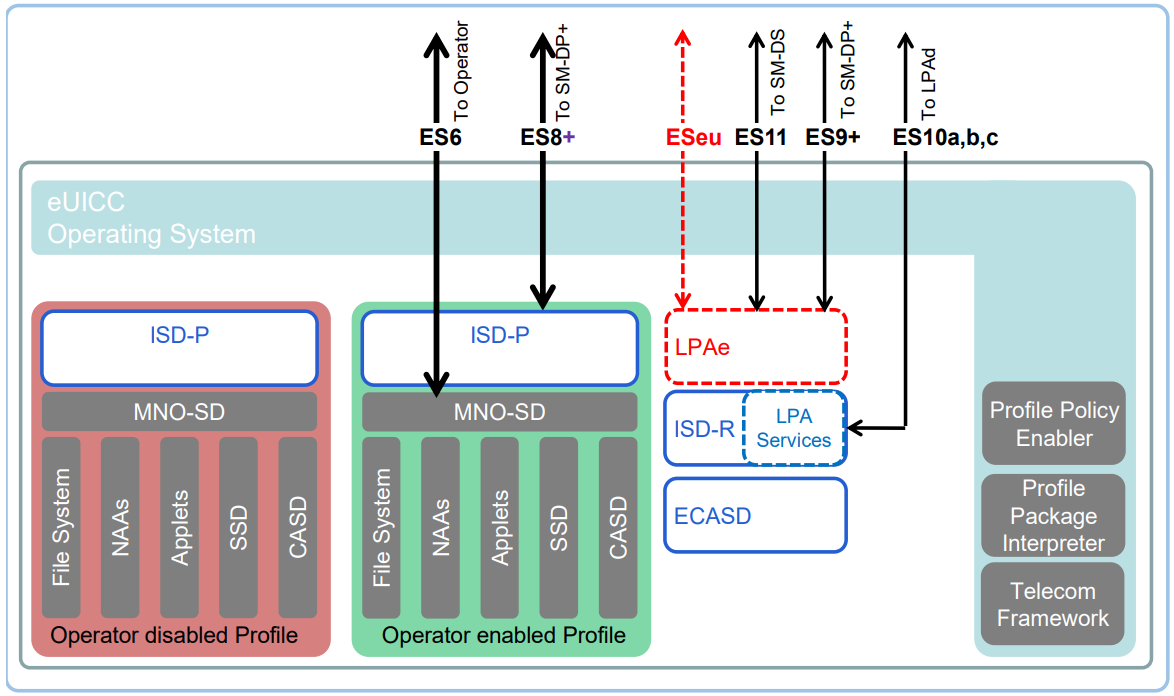
\includegraphics[width=\linewidth]{eUICC-arch.png}
\caption{Architettura dell'eUICC.}
\label{fig:eUICC-arch}
\end{figure}
\\Di seguito, invece, è riportato un breve glossario che chiarisce il significato di alcuni componenti appartenenti all'architettura dell'eUICC raffigurata in \ref{fig:eUICC-arch}.
\begin{itemize}
\item \textbf{CASD} = Controller Authority Security Domain: è un'area di storage sicura all'interno dell'ISD-P in cui vengono memorizzate le credenziali richieste per supportare le funzionalità di sicurezza sensibili.
\item \textbf{ECASD} = Embedded Controller Authority Security Domain: è il componente CASD direttamente incapsulato all'interno dell'eUICC.
\item \textbf{ISD-R} = Issuer Security Domain Root: è il componente responsabile della creazione di nuovi ISD-P e della gestione del loro ciclo di vita.
\item \textbf{LPA Services} = i seguenti quattro servizi: trasferimento del Bound Profile Package da LPAd all'ISD-P; ottenimento della lista dei profili installati; recupero dell'EID (eUICC ID); ottenimento delle operazioni di gestione del profilo locale (Local Profile Management Operations).
\item \textbf{MNO-SD} = Mobile Network Operator Security Domain: è la parte del profilo posseduta dall'operatore che fornisce all'operatore Over The Air (OTA) un canale di comunicazione sicuro; viene usato per gestire il contenuto di un profilo una volta che è stato abilitato.
\item \textbf{NAAs} = Network Access Applications: sono le applicazioni che consentono l'accesso alla rete.
\item \textbf{Profile Package Interpreter} = servizio del sistema operativo dell'eUICC che traduce i dati del Profile Package in un profilo installato all'interno dell'ISD-P codificando usando il formato interno dell'eUICC.
\item \textbf{Profile Policy Enabler} = componente che verifica che un il profilo eSIM possa essere installato sull’eUICC.
\item \textbf{SSD} = Supplementary Security Domain: è un'area di memoria protetta all'interno dell'ISD-P che viene utilizzata per l'esecuzione di funzioni di sicurezza come le operazioni crittografiche. Di fatto, il suo scopo principale è quello di proteggere le informazioni riservate dell'utente (i.e. chiavi, password) da accessi non autorizzati e attacchi esterni.
\item \textbf{Telecom Framework} = servizio del sistema operativo dell'eUICC che fornisce algoritmi di autenticazione di rete standardizzati alle applicazioni NAAs ospitate nei rispettivi ISD-P.
\end{itemize}

\subsection{Caratteristiche hardware e software dell'eUICC}
\begin{enumerate}
\item Deve essere resistente al tampering dei componenti hardware.
\item Supporta SHA-1.
\item Supporta TUAK, che è un particolare algoritmo crittografico di 3GPP, dove 3GPP (Third Generation Partnership Project) è il consorzio industriale che definisce gli standard per la tecnologia 5G .
\item Supporta Milenage, che è un set di funzioni 3GPP di autenticazione e di key generation.
\item Tutte le funzioni crittografiche devono essere resistenti al tampering e agli attacchi side-channel.
\end{enumerate}

\section{Interazione tra eUICC, LPA, SM-DP+ e operatore}
\subsection{Sicurezza TLS}
Il protocollo TLS, la cui versione 1.2 è definita in RFC 5246 \cite{RFC-5246} e la cui versione 1.3 è definita in RFC 8446 \cite{RFC-8446}, è utilizzato per proteggere il traffico sulle interfacce ES2+ (tra SM-DP+ e operatore) e ES9+ (tra SM-DP+ e LPA). In particolare, in ES2+ è prevista la mutua autenticazione tra le parti, mentre in ES9+ è prevista solo l'autenticazione del server. La documentazione di GSMA di riferimento \cite{GSMA-docs} sottolinea l'obbligatorietà di fare uso di TLS v1.2 sia per gli algoritmi di autenticazione e autorizzazione, sia per l'integrità dei messaggi, sia per la confidenzialità. In realtà, documenti più recenti di GSMA \cite{GSMA-docs2} introducono la possibilità (e suggeriscono) di utilizzare TLS v1.3, che è la versione più recente di TLS e risolve le vulnerabilità che caratterizzano TLS v1.2, per cui, in linea di principio, dovrebbe risultare particolarmente difficoltoso da penetrare. Tuttavia, attualmente sembra essere solo un suggerimento, per cui nei capitoli successivi potrebbe essere necessario verificare a livello pratico qual è la versione di TLS utilizzata per proteggere la comunicazione tra LPA e SM-DP+.

\chapter{Sicurezza dell'eSIM a run-time}
[TODO]

\chapter{Sicurezza dell'eSIM a boot-time}
\section{Funzionamento del boot dell'eSIM}
[TODO]

\section{Potenziali vulnerabilità}
[TODO]

\section{Prove sperimentali}
[TODO]

\chapter{Conclusione}
[TODO]
\cite{Android-docs}

\bibliography{Bibliography}

\chapter*{Ringraziamenti}
[TODO]

\end{document}